\documentclass{article}[13pt]

\usepackage{../../../uni-notes-eng}
\usepackage{multicol}
\definecolor{back2}{HTML}{ffffff}
\definecolor{text2}{HTML}{000000}
\usepackage{wrapfig}

\author{Weronika Jakimowicz}
\title{MDM Lista 5}
\date{}

%\pagecolor{back2}
%\color{text2}

\begin{document}
\maketitle

\section*{ZAD. 1}

Funkcja Eulera $\phi(n)$ zwraca ilość liczb względnie pierwszych z $n$.
\medskip

% Udowodnijmy pomocniczo, że jeśli $n=n_1n_2$ dla $n_1\perp n_2$, to
% $$\phi(n)=\phi(n_1)\phi(n_2).$$
% Weźmy dowolne $m$ takie, że $m\perp n$ i $m<n$. Zauważmy, że zachodzi to wtedy i tylko wtedy, gdy $m$ jest jednocześnie względnie pierwsze z $n_1$ i $n_2$. Kombinatorycznie, $m$ które to spełniają jest $\phi(n_1)\cdot\phi(n_2)$ i to daje nam wszystkie możliwości na $m$, czyli wartość $\phi(n)$.
% \medskip

% Teraz, jeśli weźmiemy $n_1=p_1^{n_1}$ oraz $n_2=\prod\limits_{i=2}^sp_i^{n_i}$, to mamy $n_1\perp n_2$ i 
% $$\phi(n)=\phi(p_1^{n_1})\phi(\prod\limits_{i=2}^sp_i^{n_i}).$$
% Możemy tę samą operację powtórzyć dla drugiego czynnika, co da nam
% $$\phi(n)=\prod\limits_{i=1}^s\phi(p_i^{n_i}).$$

Zauważmy teraz, że $n|(a^{\psi(n)}-1)$ wtw gdy $a^{\psi(n)}-1$ jest podzielne przez wszystkie elementy rozkładu $n$ na czynniki pierwsze, więc:
$$n|a^{\psi(n)}-1\iff(\forall\;i\in\{1,2,...,s\})\;p_i^{n_i}|(a^{\psi(n)}-1).$$
Tę podzielność można równoważnie wyrazić jako przystawanie $a^{\psi(n)}$ do $n$ modulo 1:
$$n|(a^{\psi(n)}-1)\iff a^{\psi(n)}\equiv 1\mod n.$$
\bigskip

Ustalmy dowolne $i$. Zauważmy, że $\phi(p_i^{n_i})|\psi(n)$, więc istnieje liczba całkowita $M$ taka, że
$$\psi(n)=\phi(p_i^{n_i})\cdot M.$$
\podz{sep}
\bigskip

Na początek chcemy pokazać twierdzenie Eulera, czyli dla dowolnego $m$ i $b\perp m$ zachodzi
$$b^{\phi(n)}\equiv 1\mod m.$$
Niech $G$ będzie grupą liczb naturalnych $p$ takich, że $0\leq p<m$ i $p\perp m$ z mnożeniem modulo $m$. W grupie tej jest $\phi(m)$ elementów. Niech $H$ będzie podgrupą cykliczną $G$ generowaną przez $b$. Wtedy rząd $H$ (czyli rząd elementu $b$) dzieli rząd $G$, bo w przeciwnym wypadku dla pewnych liczb naturalnych $k,r$, $r<o(b)$
$$e=b^{k\cdot o(b+r}=b^{k\cdot o(b)}\cdot b^{r}=(b^{o(b)})^kb^r=e\cdot b^r=b^r,$$
ale $b^r\neq e$ i mamy sprzeczność. W takim razie istnieje pewne $t$ takie, że
$$\phi(m)=o(b)\cdot t$$
i wtedy
$$b^{\phi(m)}=b^{o(b)\cdot t}=(b^{o(b)})^t=e^t=1^t=1\equiv 1\mod m.$$
\bigskip

\podz{sep}
\bigskip

Wracając do $n$, z twierdzenia Eulera mamy
$$a^{\phi(p_i^{n_1})}\equiv 1\mod p_i^{n_1}.$$
Postawmy tezę, że
$$a^{\phi(p_i^{n_i})}\equiv 1\mod n,$$
i niech $k$ będzie liczbą całkowitą, że $a^{\phi(p_i^{n_i})}=kn+1$, wtedy
$$a^{\phi(p_i^{n_i})}=kn+1=kp_i^{n_i}\prod\limits_{j=1,j\neq i}^sp_i^{n_i}+1,$$
i ponieważ $\prod\limits_{j=1,j\neq i}^sp_i^{n_i}\in\N$ daje to
$$a^{\phi(p_i^{n_i})}\equiv 1\mod n.$$
\bigskip

Ze względu na definicję funkcji $\psi(n)$ wiemy, że istnieje $M\in\N$ takie, że
$$\psi(n)=M\cdot \phi(p_i^{n_i})$$
W takim razie
$$a^{\psi(n)}=a^{M\cdot\phi(p_i^{n_i})}=(a^M)^{\phi(p_i^{n_i})}.$$
Ponieważ liczba $a$ była względnie pierwsza z $n$, to również liczba $a^M$ jest z nią względnie pierwsza, możemy ją nazwać $a^M=A\perp n$, co daje nam
$$a^{\psi(n)}=A^{\phi(p_i^{n_i})}\equiv 1\mod n.$$

\section*{ZAD. 3}

Niech $n$ będzie najwięszką z tych liczb. Chcemy pokazać, że
$$k!|n(n-1)(n-2)...(n-k+1).$$
Zauważmy, że
\begin{align*}
    n(n-1)(n-2)...(n-k+1)&={n!\over(n-k)!}=k!{n!\over(n-k)!k!}=k!{n\choose k}
\end{align*}
a dwumian Newtona dla $n,k\in\N$ jest zawsze liczbą naturalną, więc otrzymaliśmy, że dla $m={n\choose k}$
$$n(n-1)(n-2)...(n-k+1)=k!m$$

\section*{ZAD. 4}

{\color{acc}a)} Niech $n$ będzie liczbą drużyn. Każda z nich zagra dokładnie $n-1$ meczy. Czyli możemy podpisać szufladki ilością rozegranych do tej pory meczy, będzie ich $n$ sztuk. 
\smallskip

Jeżeli tylko jedna drużyna do tej pory z nikim nie grała, to nie może też się zdażyć, że któraś drużyna rozegrała wszystkie swoje mecze. Odpada więc jedna drużyna i szufladki podpisane 0 i $n-1$, co zostawia nas z $n-1$ drużynami pakowanymi do $n-2$ szufladek, więc dwie wpadną do jednej szufladki i będą miały taką samą ilość meczów.
\smallskip

Jeżeli każda drużyna rozegrała co najmniej jeden mecz, to odpada nam szufladka podpisana 0. Mamy więc $n-1$ szufladek i $n$ drużyn, z czego wynika że dwie mają tę samą ilość rozegranych meczy.
\medskip

{\color{acc}b)} Podzielmy trójkąt równoboczny na 4 trójkąty tak, jak na ilustracji obok.
\begin{wrapfigure}{r}{0.25\textwidth}
    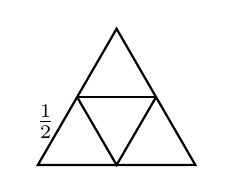
\begin{tikzpicture}
        \coordinate (A) at (-1, 0);
        \coordinate (B) at (1, 0);
        \coordinate (C) at (0, 1.73);

        \coordinate (D) at (-0.5, 0.86);
        \coordinate (E) at (0.5, 0.86);
        \coordinate (F) at (0, 0);
    
        \draw[thick] (A)--(B)--(C)--cycle;
        \draw[thick] (D)--(E);

        \draw[thick] (E)--(F)--(D);

        \node at (-0.9, 0.55) {$\frac12$};
    \end{tikzpicture}
\end{wrapfigure}
Dostajemy 4 trójkątów równobocznych o boku $\frac12$. Odległość dwóch dowolnych punktów znajdujących się w obrębie jednego z tych małych trójkątów jest co najwyżej $\frac12$. Wybierając 5 losowych punków w dużym trójkącie mamy pewność, że co najmniej dwa będą usytuowane w obrębach jednego małego trójkąta, a więc odległość między nimi nie przekroczy $\frac12$.
\medskip

{\color{acc}c)} Niech $n$ będzie ilością ścian w wielościanie wypukłym. Każda ściana ma między $3$ (czworościan) a $n-1$ sąsiadów. Ilość sąsiadów ściany to również ilość jej krawędzi. Mamy $n-3$ szufladki i $n$ ścian do rozłożenia między nie, więc na pewno stanie się, że dwie wylądują w jednej szufladce i będą miały równą ilość krawędzi.

\section*{ZAD. 5}

Jeżeli jedna z liczb jest podzielna przez $n$, to zadanie jest trywialne. Rozważmy więc sytuację, kiedy żadna z liczb $a_1,..., a_n$ nie jest podzielna przez $n$. Zauważmy, że wtedy reszta z dzielenia każdej z tych liczb przez $n$ jest co najmniej 1 i co najwyżej $n-1$.
\smallskip

Oznaczmy przez $S_k$ sumy częściowe tych liczb:
$$S_k=\sum\limits_{i=1}^k a_i.$$
Reszta z dzielenia $S_k$ przez $n$ wpada pomiędzy $0$ a $n-1$. Znowu, jeśli trafi nam się suma częściowa podzielna przez $0$, to kończymy. W przeciwnym wypadku dostajemy szufladki podpisane resztami od $1$ do $n-1$, co daje $n-1$ szufladek na $n$ sum. W takim razie dwie różne sumy mają tę samą resztę z dzielenia przez $n$, niech to będą $S_j$ i $S_k$, $j>k$. Ich różnica $S_j-S_k$ jest podzielna przez $n$, a wynosi
$$S_j-S_k=\sum\limits_{i=1}^js_i-\sum\limits_{i=1}^ka_i=\sum\limits_{i=k}^ja_i$$
i to jest koniec.

\section*{ZAD. 6}

Jeśli dwie liczby się powtarzają, to oczywiście wystarczy wziąć dwa singletony tych powtarzających się liczb. Przyjmijmy więc, że taka sytuacja nie ma miejsca.
\smallskip

Spośród 10 liczb możemy wybierać niepuste podzbiory na 
$$2^{10}-1=1023$$ 
sposobów, bo zbiór potęgowy zbioru $10$ elementowego ma $2^{10}$ elementów, ale my nie chcemy zbioru pustego z oczywistych przyczyn.
\smallskip

Suma $s$ podzbioru 10 różnych liczb naturalnych jest pomiędzy
\begin{align*}
    1\leq s\leq 945=\sum\limits_{i=1}^{10}(89+i)
\end{align*}
więc mamy $943$ możliwych wartości $s$, a dla dowolnego zbioru $S$ możemy takich wartości wyprodukować $1023$. W takim razie co najmniej dwie z nich mają tę samą sumę.


\section*{ZAD. 7}

Mamy dane $nk+r$ kulek i $n$ szuflad, gdzie $0\leq r$ i $s<n$. Chcemy szufladę w której jest co najmniej $sk+\min(r,s)$ kulek.
\smallskip

Rozważmy najgorszy przypadek, czyli kiedy rozkładamy kulki tak bardzo równo jak się da. Niech w ostatnich szufladkach będzi więcej kulek, wtedy w $i$-tej szufladce dostajemy
$$\lfloor{nk+r+i\over n}\rfloor=\lfloor k+{r+i\over n}\rfloor=k+\lfloor{r+i\over n}\rfloor$$
kulek, co udowadniałam w zadaniu 2 na liście 2. Zadanie sprowadza się do pokazania, że możemy wybrać taki ciąg $i_1,...,i_s$, że
$$\sum\limits_{k=1}^s\lfloor{r+i_k\over n}\rfloor=\min(r,s).$$

Zauważy, że jeśli $r<n$, to dokładnie $n-r$ tych wartości jest równe zero, natomiast pozostałe $r$ jest równe 1. Teraz, jeśli $s<r$, to wystarczy wziąc $s$ szufladek z dodatkową piłeczką, a w przeciwnym wypadku wystarczy wziąć wszystkie $r$ szufladek z dodatkową piłeczką i $s-r$ szufladek bez dodatkowej piłeczki. 

W przeciwnym wypadku $r\geq n$, więc $s<r$ i wtedy każda szufladka ma co najmniej $k+1$ piłeczek, więc dowolne $s$ szufladek ma ich co nie mniej niż $sk+s$.

\section*{ZAD. 8}

Mamy szachownicę o $n$ wierszach i $m$ kolumnach. Wieże na szachownicy nie atakują się, jeśli nie są ani w jednej kolumnie ani w jednym wierszu. Mamy więcej kolumn, więc ograniczają nas tak naprawdę wiersze, których jest $n$. Jeśli więc będziemy wymagać $n+1$ wież które sa w różnych wierszach i kolumnach, to nam się nie uda, bo co najmniej dwie znajdą się w jednym wierszu. W takim razie 
$$k\leq n.$$

Ponumerujmy "przekątne" planszy kolejnymi liczbami naturalnymi. Przez przekątną rozumiem tutaj zbiór pól takich, że możemy przejść po ukosie stykając się rogami z góry w dół w prawo (zielona), albo możemy dojść do prawej krawędzi planszy i przeskakujemy na początek i dochodzimy na dół (pomarańczowa).
\begin{center}
    \begin{tikzpicture}
        \filldraw[color=acc, fill=acc] (1, 4) rectangle (2, 3);
        \filldraw[color=acc, fill=acc] (2, 3) rectangle (3, 2);
        \filldraw[color=acc, fill=acc] (3, 2) rectangle (4, 1);
        \filldraw[color=acc, fill=acc] (4, 1) rectangle (5, 0);

        \filldraw[color=def, fill=def] (0, 1) rectangle (1, 0);
        \filldraw[color=def, fill=def] (3, 4) rectangle (4, 3);
        \filldraw[color=def, fill=def] (4, 3) rectangle (5, 2);
        \filldraw[color=def, fill=def] (5, 2) rectangle (6, 1);
        \foreach \x in {0,...,6}
            \foreach \y in {0,...,4}
                \coordinate (\x\y) at (\x,\y);
        
        \foreach \x in {0,...,6}
            \foreach \y [count=\yi] in {0,...,3}
                \draw (\x\y)--(\x\yi);
        
        \foreach \y in {0,...,4}
            \draw (0\y)--(6\y);
            
        
    \end{tikzpicture}
\end{center}

Takich przekątnych mamy $m$, bo dla każdego pola na górnej krawędzi planszy mamy unikalną przekątną. Zauważmy, że wieże nie szachują się, jeśli stoją wszystkie na takiej jednej przekątnej. Mamy $m(k-1)+1$ wież. Rozkładając pierwsze $m(k-1)$ jak najbardziej równo dostaniemy po $k-1$ wież w każdej przekątnej. Ostatnia wieża może więc trafić do dowolnej przekątnej i na niej będzie $k$ wież które się nie biją.

\end{document}